\documentclass[aspectratio=169, xcolor=dvipsnames]{beamer}

% --- Theme Setup ---
\usetheme{Madrid}
\usecolortheme{default}

% --- Packages ---
\usepackage{graphicx}
\usepackage{xcolor}
\usepackage{booktabs}
\usepackage{hyperref}
\usepackage{adjustbox}
\usepackage{amssymb}
\usepackage{amsmath}
\usepackage{listings}
\usepackage{caption}

\lstset{
  basicstyle=\ttfamily\small,
  keywordstyle=\color{blue}\bfseries,
  stringstyle=\color{red},
  showstringspaces=false,
  breaklines=true
}

% --- Title Information ---
\title{Module 09}
\subtitle{Introduction to SQL/2}
\author{Milav Dabgar}
\institute{www.milav.in}
\date{\today}

\begin{document}

% Title Slide
\begin{frame}
    \titlepage
\end{frame}

\begin{frame}{Module Recap}
    \begin{itemize}[<+->]
        \item Introduced relational query language
        \item Familiarized with data definition and basic query structure
    \end{itemize}
\end{frame}

\begin{frame}{Module Objectives}
    \begin{block}{Goals}
        \begin{itemize}[<+->]
            \item To understand Cartesian Product
            \item To familiarize with String operations
            \item To familiarize with Ordering and set operations
        \end{itemize}
    \end{block}
\end{frame}

\begin{frame}{Module Outline}
    \begin{itemize}[<+->]
        \item Cartesian Product
        \item Joins
        \item Rename Operation
        \item String Operations
        \item Ordering
        \item Set Operations
    \end{itemize}
\end{frame}

\section{Additional Basic Operations}

\begin{frame}
  \vfill
  \centering
  \begin{beamercolorbox}[sep=8pt,center,shadow=true,rounded=true]{title}
    \usebeamerfont{title}Additional Basic Operations\par%
  \end{beamercolorbox}
  \vfill
\end{frame}

\begin{frame}[fragile]{Cartesian Product}
    \begin{itemize}
        \item Find the Cartesian product \texttt{instructor $\times$ teaches}
        \begin{lstlisting}[language=SQL]
select * 
from instructor, teaches;
        \end{lstlisting}
        \item generates every possible instructor-teaches pair, with all attributes from both relations
        \item For common attributes (for example, \texttt{ID}), the attributes in the resulting table are renamed using the relation name (for example, \texttt{instructor.ID})
        \item Cartesian product not very useful directly, but useful combined with \texttt{where}-clause condition (selection operation in relational algebra)
    \end{itemize}
\end{frame}

\begin{frame}{Cartesian Product - Illustration}
    \begin{center}
        \textbf{instructor} \qquad $\times$ \qquad \textbf{teaches} \\
        \vspace{1em}
        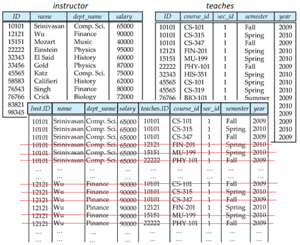
\includegraphics[height=0.6\textheight, width=0.9\textwidth, keepaspectratio]{../Lecture 2.4_artifacts/image_000008_87d16a7ad0a40dee62ec6ed38194a669ec256e60edfccb1cc899bf5641f5af7b.png}
    \end{center}
\end{frame}

\begin{frame}{Joins}
    \begin{block}{Overview}
        \begin{itemize}[<+->]
            \item For all instructors who have taught some course, find their names and the course ID of the courses they taught
            \item We can write:
            \begin{center}
                \texttt{select name, course\_id \\
                        from instructor, teaches \\
                        where instructor.ID = teaches.ID}
            \end{center}
            \item Find the course ID, semester, year and title of each course offered by the Comp. Sci. department
            \label{cs_dept_query}
            \begin{center}
                \texttt{select section.course\_id, semester, year, title \\
                        from section, course \\
                        where section.course\_id = course.course\_id and dept\_name = 'Comp. Sci.'}
            \end{center}
        \end{itemize}
    \end{block}
\end{frame}

\begin{frame}{Rename Operation}
    \begin{block}{Overview}
        \begin{itemize}[<+->]
            \item The SQL allows renaming relations and attributes using the \texttt{as} clause:
            \begin{center}
                \texttt{old-name as new-name}
            \end{center}
            \item Example:
            \begin{center}
                \texttt{select ID, name, salary/12 as monthly\_salary \\
                        from instructor}
            \end{center}
            \item Find the names of all instructors who have a higher salary than some instructor in 'Comp. Sci'.
            \begin{center}
                \texttt{select distinct T.name \\
                        from instructor as T, instructor as S \\
                        where T.salary > S.salary and S.dept\_name = 'Comp. Sci.'}
            \end{center}
            \item Keyword \texttt{as} is optional and may be omitted.
            \begin{center}
                \texttt{instructor as T $\equiv$ instructor T}
            \end{center}
        \end{itemize}
    \end{block}
\end{frame}

\begin{frame}{Cartesian Product Example}
    \begin{itemize}
        \item Relation \texttt{emp\_super}
        \item Find the supervisor of 'Bob'
        \item Find the supervisor of the supervisor of 'Bob'
        \item Find ALL the supervisors (direct and indirect) of 'Bob'
    \end{itemize}
    \vspace{1em}
    \begin{center}
        \begin{adjustbox}{max width=\textwidth}
        \begin{tabular}{|l|l|}
        \hline
        \textbf{person} & \textbf{supervisor} \\ \hline
        Bob & Alice \\ \hline
        Alice & Susan \\ \hline
        David & David \\ \hline
        Mary & Mary \\ \hline
        \end{tabular}
        \end{adjustbox}
    \end{center}
\end{frame}

\begin{frame}{String Operations}
    \begin{block}{Pattern Matching}
        \begin{itemize}[<+->]
            \item SQL includes a string-matching operator for comparisons on character strings. The operator \texttt{like} uses patterns that are described using two special characters:
            \begin{itemize}
                \item[$\triangleright$] \texttt{\%} (percent): The \% character matches any substring.
                \item[$\triangleright$] \texttt{\_} (underscore): The \_ character matches any character.
            \end{itemize}
            \item Find the names of all instructors whose name includes the substring ``dar''.
            \begin{center}
                \texttt{select name \\
                        from instructor \\
                        where name like '\%dar\%'}
            \end{center}
            \item Match the string \texttt{"100 \%"}
            \begin{center}
                \texttt{like '100 \textbackslash\%' escape '\textbackslash'}
            \end{center}
        \end{itemize}
    \end{block}
\end{frame}

\begin{frame}{String Operations (2)}
    \begin{itemize}[<+->]
        \item Patterns are case sensitive.
        \item Pattern matching examples:
        \begin{itemize}
            \item[$\triangleright$] \texttt{'Intro\%'} matches any string beginning with \texttt{"Intro"}.
            \item[$\triangleright$] \texttt{'\%Comp\%'} matches any string containing \texttt{"Comp"} as a substring, for example, \texttt{"Intro. to Comp. Sci."}, and \texttt{"Comp. Sci. and Engg."}.
            \item[$\triangleright$] \texttt{'\_\_\_'} matches any string of exactly three characters.
            \item[$\triangleright$] \texttt{'\_\_\_\%'} matches any string of at least three characters.
        \end{itemize}
        \item SQL supports a variety of string operations such as
        \begin{itemize}
            \item[$\triangleright$] concatenation (using $\mid\mid$)
            \item[$\triangleright$] converting from upper to lower case (and vice versa)
            \item[$\triangleright$] finding string length, extracting substrings, etc.
        \end{itemize}
    \end{itemize}
\end{frame}

\begin{frame}{Ordering the Display of Tuples}
    \begin{block}{Order By}
        \begin{itemize}[<+->]
            \item List in alphabetic order the names of all instructors
            \begin{center}
                \texttt{select distinct name \\
                        from instructor \\
                        order by name}
            \end{center}
            \item We may specify \texttt{desc} for descending order or \texttt{asc} for ascending order, for each attribute; ascending order is the default.
            \begin{itemize}
                \item[$\triangleright$] Example: \texttt{order by name desc}
            \end{itemize}
            \item Can sort on multiple attributes
            \begin{itemize}
                \item[$\triangleright$] Example: \texttt{order by dept\_name, name}
            \end{itemize}
        \end{itemize}
    \end{block}
\end{frame}

\begin{frame}[fragile]{Selecting Number of Tuples in Output}
    \begin{itemize}
        \item The \texttt{Select Top} clause is used to specify the number of records to return
        \item The \texttt{Select Top} clause is useful on large tables with thousands of records. Returning a large number of records can impact performance
        \begin{lstlisting}[language=SQL]
select top 10 distinct name 
from instructor;
        \end{lstlisting}
        \item Not all database systems support the \texttt{SELECT TOP} clause.
        \begin{itemize}
            \item SQL Server \& MS Access support \texttt{select top}
            \item MySQL supports the \texttt{limit} clause
            \item Oracle uses \texttt{fetch first n rows only} and \texttt{rownum}
        \end{itemize}
        \begin{lstlisting}[language=SQL]
select distinct name 
from instructor 
order by name 
fetch first 10 rows only;
        \end{lstlisting}
    \end{itemize}
\end{frame}

\begin{frame}{Where Clause Predicates}
    \begin{block}{\texttt{between} operator}
        \begin{itemize}[<+->]
            \item SQL includes a \texttt{between} comparison operator
            \item Example: Find the names of all instructors with salary between \$90,000 and \$100,000 (that is, $\geq \$90,000$ and $\leq \$100,000$)
            \begin{center}
                \texttt{select name \\
                        from instructor \\
                        where salary between 90000 and 100000}
            \end{center}
            \item Tuple comparison
            \begin{center}
                \texttt{select name, course\_id \\
                        from instructor, teaches \\
                        where (instructor.ID, dept\_name) = (teaches.ID, 'Biology');}
            \end{center}
        \end{itemize}
    \end{block}
\end{frame}

\begin{frame}[fragile]{In Operator}
    \begin{itemize}
        \item The \texttt{in} operator allows you to specify multiple values in a \texttt{where} clause
        \item The \texttt{in} operator is a shorthand for multiple \texttt{or} conditions
        \begin{lstlisting}[language=SQL]
select name
from instructor
where dept_name in ('Comp. Sci.', 'Biology');
        \end{lstlisting}
    \end{itemize}
\end{frame}

\begin{frame}{Duplicates}
    \begin{itemize}
        \item In relations with duplicates, SQL can define how many copies of tuples appear in the result
        \item Multiset versions of some of the relational algebra operators - given multiset relations $r_1$ and $r_2$:
        \begin{itemize}
            \item[a)] $\sigma_{\theta}(r_1)$: If there are $c_1$ copies of tuple $t_1$ in $r_1$, and $t_1$ satisfies selections $\sigma_{\theta}$, then there are $c_1$ copies of $t_1$ in $\sigma_{\theta}(r_1)$
            \item[b)] $\Pi_A(r_1)$: For each copy of tuple $t_1$ in $r_1$, there is a copy of tuple $\Pi_A(t_1)$ in $\Pi_A(r_1)$ where $\Pi_A(t_1)$ denotes the projection of the single tuple $t_1$
            \item[c)] $r_1 \times r_2$: If there are $c_1$ copies of tuple $t_1$ in $r_1$ and $c_2$ copies of tuple $t_2$ in $r_2$, there are $c_1 \times c_2$ copies of the tuple $t_1 \cdot t_2$ in $r_1 \times r_2$
        \end{itemize}
    \end{itemize}
\end{frame}

\begin{frame}{Duplicates (2)}
    \begin{itemize}
        \item Example: Suppose multiset relations $r_1(A, B)$ and $r_2(C)$ are as follows: 
        \begin{center}
            $r_1 = \{(1, a), (2, a)\}$ \\
            $r_2 = \{(2), (3), (3)\}$
        \end{center}
        \item Then $\Pi_B(r_1)$ would be $\{(a), (a)\}$, while $\Pi_B(r_1) \times r_2$ would be $\{(a, 2), (a, 2), (a, 3), (a, 3), (a, 3), (a, 3)\}$
        \item SQL duplicate semantics:
        \begin{center}
            \texttt{select $A_1, A_2, \dots, A_n$ \newline from $r_1, r_2, \dots, r_m$ \newline where $P$}
        \end{center}
        \item Is equivalent to the multiset version of the expression:
        \begin{center}
            $\Pi_{A_1, A_2, \dots, A_n} (\sigma_P (r_1 \times r_2 \times \dots \times r_m))$
        \end{center}
    \end{itemize}
\end{frame}

\begin{frame}{Module Summary}
    \begin{itemize}
        \item Completed the understanding of basic query structure
    \end{itemize}
    \vspace{2em}
    \begin{center}
    \small \textit{Slides used in this presentation are borrowed from \url{http://db-book.com/} with kind permission of the authors.} \\
    \small \textit{Edited and new slides are marked with 'PPD'.}
    \end{center}
\end{frame}

\end{document}
